\documentclass[11pt,a4paper,oneside]{article}
\usepackage{titling}
\newcommand{\subtitle}[1]{%
  \posttitle{%
    \par\end{center}
    \begin{center}\large#1\end{center}
    \vskip0.5em}%
}
\title{\textbf{Group 21: Cognitive Modeling - Lab 3}}
\date{\today}
\author{Olusanmi Hundogan - 6883273\\
Evangelia Giannikou - 6988229\\
}
% \pagenumbering{gobble}
\pagenumbering{arabic}

% \usepackage{eurosym}
\usepackage{hyperref}
% \usepackage{subfig}
\usepackage{amsmath}
\usepackage{amssymb}
\usepackage{tabularx,booktabs}
\usepackage{multicol}
\usepackage{array}
\usepackage{float}
\usepackage[english]{babel}
\usepackage{wrapfig}
\usepackage{graphicx}
\usepackage[font=scriptsize]{caption}
\usepackage{subcaption}


\setcounter{secnumdepth}{0}
\newcolumntype{M}[1]{>{\centering\arraybackslash}m{#1}}
\usepackage[backend=biber, sorting=none]{biblatex}
\usepackage[margin=1in]{geometry}
\addbibresource{references.bib}

\newcommand{\icol}[1]{% inline column vector
  \left(\begin{smallmatrix}#1\end{smallmatrix}\right)%
}

\newcommand{\irow}[1]{% inline row vector
  \begin{smallmatrix}(#1)\end{smallmatrix}%
}

\begin{document}

\maketitle

\section{Question 1}
\label{Q1}
\subsection{Height: mean = 180, st.d = 10}
\textit{Show two graphs: (i) what the \textbf{probability} of using threshold looks like on the scale 1-250 cm; (ii) the graph of the function $\sigma$ on the same scale. State which degree point has the highest probability of being used as a threshold, and on which degree point it is most likely the speaker will use the adjective tall. If the two values differ or are the same, say in a few words why you think this is so.}\\

In Figure \ref{fig:q1_threshold}, the \textbf{probability} of using threshold on the scale 1-250 cm is shown. The highest degree point is when $ P(\Theta; \lambda; c) = 0.083$, and $\theta = 184$ cm.

\begin{figure}[H]
    \centering
    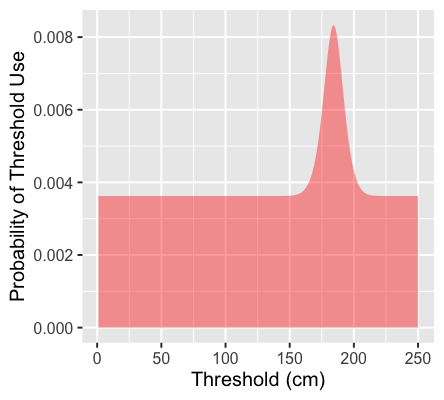
\includegraphics[width=100mm]{figs/Question_1_threshold.png}
    \caption{The graph shows the utility of threshold U on a scale of 1-250 cm.}
  \label{fig:q1_threshold}
\end{figure}

Similarly, in Figure \ref{fig:q1_sigma}, it is shown the graph of the function $\sigma$ on the same x-scale. The highest degree point is 1 and height = 250 cm. 250 yields the highest likelihood of adjective use. At this threshold, it is certain that if the speaker utters "tall" he will be referring to 250 and the listener will understand it as such. As the value decreases, the likelihood is diminishing as well.

\begin{figure}[H]
    \centering
    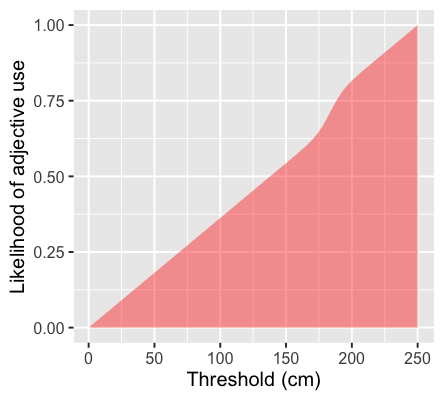
\includegraphics[width=100mm]{figs/Question_1_sigma.png}
    \caption{The graph shows the function $\sigma$ on a scale 1-250 cm.}
  \label{fig:q1_sigma}
\end{figure}

Comparing the two degree points to evaluate the communication efficiency, it is evident that the two values deviate. Considering that $\theta = 255$ is optimal, the speaker is most likely to use the adjective "tall" for heights greater than 184 cm when $\theta = 0.083$. For lower values of $\theta$, someone described as "tall" does not indicate a lot about the actual height , making it inefficient to use the adjective.

\section{Question 2}
\label{Q2}
\subsection{IQ - normal distribution}
\textit{Specify the normal distribution and generate figures for $ES$ and $\sigma$ function using this distribution and report which degree has the highest $ES$.}\\

For specifying the IQ distribution, we use $IQ \sim \mathcal{N}(100, 15)$ since $mean = 100$, given from the description, and with 95\% confidence interval $st.d. = 15$. 

\begin{figure}[H]
    \centering
    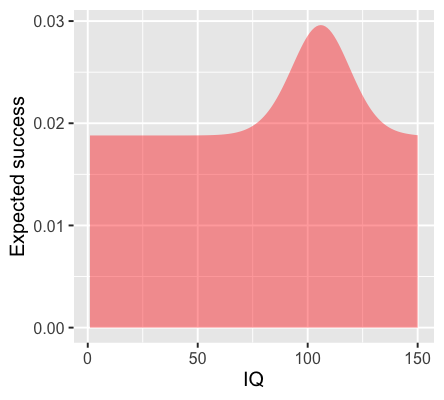
\includegraphics[width=100mm]{figs/Question_2_IQ_es.png}
    \caption{The graph shows the Expected Success function for IQ on a scale of 1-150.}
  \label{fig:q2_iq_es}
\end{figure}

The highest degree in Figure \ref{fig:q2_iq_es} is when $ES = 0.029$ for $IQ = 106$.


\begin{figure}[H]
    \centering
    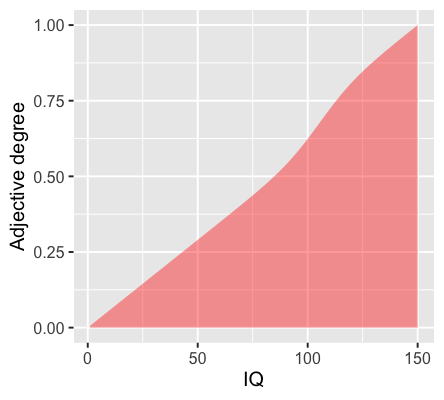
\includegraphics[width=100mm]{figs/Question_2_IQ_sigma.png}
    \caption{The graph shows the $\sigma$ function for IQ on a scale of 1-150.}
  \label{fig:q2_iq_sigma}
\end{figure}

The highest degree in Figure \ref{fig:q2_iq_sigma} is when $ES = 1$ for $IQ = 150$.


\subsection{Waiting times - gamma distribution}
\textit{Specify the gamma distribution and generate figures for $ES$ and $\sigma$. Report which degree has the highest $ES$.}\\

For specifying the waiting times distribution, we use Waiting times $\sim \mathcal{\gamma}(2, 1)$. 
%[TO-DO: explain more why these values]

\begin{figure}[H]
    \centering
    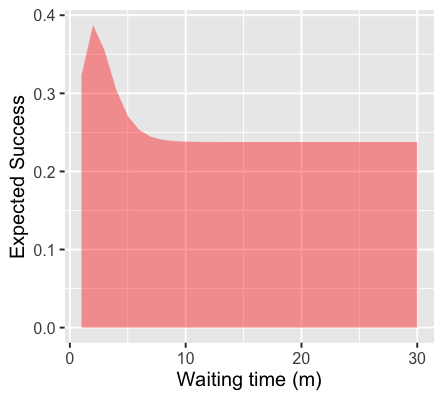
\includegraphics[width=100mm]{figs/Question_2_waiting_time_es.png}
    \caption{The graph shows the $\sigma$ function for waiting on a scale of 1-30.}
  \label{fig:q2_waiting_es}
\end{figure}
The highest degree in Figure \ref{fig:q2_waiting_es} is when $ES = 0.387$ for waiting time $= 2$ minutes.


\begin{figure}[H]
    \centering
    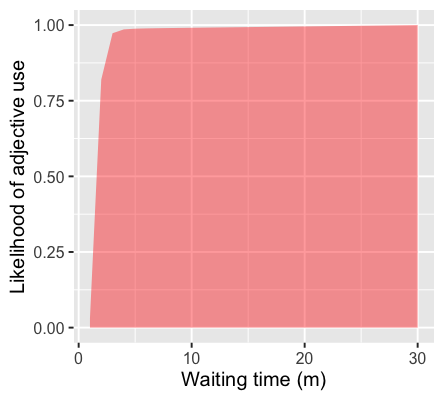
\includegraphics[width=100mm]{figs/Question_2_waiting_time_sigma.png}
    \caption{The graph shows the $\sigma$ function for waiting on a scale of 1-30.}
  \label{fig:q2_waiting_sigma}
\end{figure}
The highest degree in Figure \ref{fig:q2_waiting_sigma} is when $ES = 1$ for waiting time $= 30$ minutes.


\section{Question 3}
\label{Question 3}
\textit{What is Pearson’s correlation coefficient, r, between model’s predictions and actual observations. Check the value of $r$ with respect to three different parameters of the model (9 comparisons in total):}

\begin{itemize}
    \item \textit{lambda=40, coverage.parameter=0.1}
    \item \textit{lambda=40, coverage.parameter=-0.1}
    \item \textit{lambda=40, coverage.parameter=0}
\end{itemize}

\textit{What coverage parameter gives us the best and the worst linear correlation? On which distribution do we get the best results?}

\textit{Afterward, pick the coverage parameter that worked best and select two distributions by flipping their prior belief distributions. Report what prior distribution you used and report r. Do we see that r is affected? Does the model suffer in having worse linear correlation with respect to the observed data? Say in a few words why this is the case.}\\

As it is visible in Table \ref{question_3}, the best linear correlation is given when the coverage parameter is -0.1 where on average $r = 0.97$. The worst correlation is given when coverage parameter is 0.1 where on average $r = 0.86$.

Similarly, when comparing the results between the distribution, the best correlation is that of the Left-skewed with an average $r = 0.94$. The worst correlation is given for the Moved distribution where on average $r = 0.91$.

\begin{table}[ht]
\centering
\begin{tabular}{rccc}
  \hline
 Model & r when $c = 0.1$ & r when $c = -0.1$ & r when $c = 0$ \\ 
  \hline
    Gaussian & 0.88 & 0.97 & 0.94\\ 
    Left - skewed & 0.85 & 0.98 & 0.98\\ 
    Moved & 0.84 & 0.97 & 0.93\\ 
   \hline
\end{tabular}
\caption{Pearson's correlation between model's prediction and actual observation for 3 different model distributions where $\lambda = 40$ and coverage parameter is 0.1, -0.1 and 0.}
\label{question_3}
\end{table}

For the second part of the question, we picked $c = -0.1$ as the best coverage parameter and selected to flip the distribution of the left-skewed and moved models. In particular, we used $\mathcal{N}(6, 2)$ for the left-skewed model. The correlation we found was $r = 0.95$. For the moved model we used $\mathcal{\gamma}(4, 1.5)$. The correlation found was $r = 0.86$.

A sum of the results in regards to the previously observed data is found on Table \ref{question_3_flipped}. In the case of the left-skewed model, the correlation worsens slightly with a prior distribution set. This decrease was expected since gamma distribution would not work well with data that are concentrated on the right side of distribution. In contrast, for the moved model, the correlation improves a lot. 
% [TO-DO: explain why this happens even more?!]

\begin{table}[ht]
\centering
\begin{tabular}{rccr}
  \hline
 Model & r with Normal distribution & r with Gamma distribution\\ 
  \hline
    Left - skewed & 0.95* & 0.98 \\ 
    Moved & 0.97 & 0.86* \\ 
   \hline
\end{tabular}
\caption{Pearson's correlation between 2 models with $c = -0.1$. R values with * indicate the new correlation values with flipped distribution.}
\label{question_3_flipped}
\end{table}

\section{Question 4} 
\label{Question 4}
\textit{Bayesian model - What values have been found for lambda and coverage.parameter? Report summary statistics on lambda and coverage.parameter (MAP, median, 2.5\% to 97.5\%). Discuss briefly the summaries.}\\

For the Bayesian model, we used as a prior $\mathcal{N}(6, 2)$. As seen in Table \ref{question_4},  the values of 2.5\% and 97.5\% interval indicate the limits of c and $\lambda$. Hence, there is a 95\% chance that $ c \in [-0.332, -0.107]$ and $\lambda \in [18.483, 48.985]$. The MAP values are $c = -0.197$ and $\lambda = 33.364$. These values are very close to the ones we used in \autref{Question 3} ($\lambda = 40$, $c = -0.1$). The correlation there had the highest value for a Gaussian distribution, which is used here as a prior.

%[TO-DO: should we also say, that because the values are close the ones from the previous question, it means that the Bayesian model will have good results ?! sth like that ]

\begin{table}[ht]
\centering
\begin{tabular}{ccccc}
  \hline
  & MAP & median & 2.5\% interval & 97.5\% interval\\ 
  \hline
    c & -0.197 & -0.204 & -0.332 & -0.107\\ 
    $\lambda$ & 33.364 & 34.919 & 18.483 & 48.985\\ 
   \hline
\end{tabular}
\caption{A statistics summary of c and $\lambda$ for adjective='big' on a Gaussian distribution.}
\label{question_4}
\end{table}


\section{Question 5}
\label{Q5}
\textit{Expand your model to construct the posterior distribution of the two parameters using three adjectives (big, pointy, tall) in all three distributions. Explore the distribution of the parameters in out. Plot the summary and report summary statistics on lambda and coverage.parameter.}\\

Similar to \autref{Question 4}, we used as a prior $\mathcal{N}(6, 2)$ for all three adjectives 'big','pointy' and 'tall'. Again, there is a 95\% chance that $ c \in [-0.080, -0.028]$ and $\lambda \in [23.653, 47.599]$. The MAP values are $c = -0.051$ and $\lambda = 32.840$ which are further away from $c = -0.01$ and $\lambda = 40$. In addition, these values are worse than previously, which is expected since we extended the model in order to make predictions for 3 adjectives that are different.

\begin{table}[ht]
\centering
\begin{tabular}{ccccc}
  \hline
  & MAP & median & 2.5\% interval & 97.5\% interval\\ 
  \hline
    c & -0.051 & -0.052 & -0.080 & -0.028\\ 
    $\lambda$ & 32.840 & 34.614 & 23.653 & 47.599\\ 
   \hline
\end{tabular}
\caption{A statistics summary of c and $\lambda$ for adjectives = 'big', 'pointy', 'tall' for 3 distributions.}
\label{question_5}
\end{table}

\section{Bonus question}
\label{bonus}
\textit{We specified the likelihood using dnorm with $sd=0.1$. Is this sensible or not? Check what dnorm is and state what problems there might be with this particular function and with $sd=0.1$ for our data. Is there an alternative probability distribution that would make more sense?}\\

Standard deviation shows how much variation or "dispersion" there is from the mean. A low value of st.d. as here, indicate that the data points tend to be close to the mean. By keeping the data points concentrated to the mean, we ensure that the likehood's values will not be widespread. 

%the accuracy of someone using an adjective ?!

A left-skewed distribution might be better to use. Firstly because we tested the distributions on the previous question and proved that left-skewed had a better correlation value.

Second, because we want to ensure the communication efficiency. In a left-skewed distribution, small data values are gathered on the left, whereas higher values are gathered to the right. Communication efficiency increases as the values of likelihood increase. Since we want a concentration of values on the ride side to increase communication efficiency, a left skewed distribution might be a better choice.

\clearpage 
\printbibliography
\end{document}